\chapter{Theory}
\label{sec:theory}
This chapter will explain what \hyperref[sec:terahertz]{terahertz} radiation is, how to generate it through \hyperref[sec:optic_ref]{optical rectification}, and the detection through \hyperref[sec:eos]{electro-optic sampling}.
Furthermore, the calculation of the terahertz electric field and its power will be presented in section \ref{sec:eos}.
\section{Terahertz radiation}
\label{sec:terahertz}
This thesis will show the means of generating terahertz ($\si{\tera\hertz}$) radiation, with two non-linear crystals.
As the name describes, its frequency regime lies at about \\${(0.3-30)\cdot10^{12}\,\si{\hertz}}$.
Its wavelength can be calculated by
\begin{equation}
    \lambda = \frac{c}{\nu}
\end{equation}
with the speed of light $c$ and its frequency $\nu$, which results in a wavelength of about $\SI{100}{\micro\meter}-\SI{1}{\milli\meter}$.
This means it lies between infrared and microwave radiation.
$\si{\tera\hertz}$ radiation is caused by various linear and non-linear effects which only occur at relatively high powers \cite{Thz_sources}.
The need for high powers, as well as the lack of emitters, makes it hard to generate it efficiently.
The result is the so-called $\si{\tera\hertz}$ gap that is slowly being closed by new techniques and advances in science.
Some of these are the generation of $\si{\tera\hertz}$ radiation through organic and inorganic crystals, as well as the use of semiconductors \cite{sources_thz}.
\\
$\si{\tera\hertz}$ radiation is non-ionizing but is absorbed by water \cite{water_absorption}.
This makes it of particular interest for medical uses.
The water absorption will be shown later. 
%%%%%%%%%%%%%%%%%%%%%%%%%%%%%%%%%%%%%%%%%%%%%%%%%%%%%%%%%%%%%%%%%%%%%%%%%%%%%%%%%%


%%%%%%%%%%%%%%%%%%%%%%%%%%%%%%%%%%%%%%%%%%%%%%%%%%%%%%%%%%%%%%%%%%%%%%%%%%%%%%%%%%
\section{Terahertz emitters}
\label{sec:emitters}
There are different kinds of $\si{\tera\hertz}$ emitters, such as photoconductive antennas, and organic and inorganic crystals \cite{Tutorial}.
These emitters all have advantages and disadvantages, which makes them more useful for some applications than others.
$\si{\tera\hertz}$ emitters such as photoconductive antennas generate a narrowband spectrum, which is not tunable \cite{PCA_bandwidth}.
This makes them suitable for more specialized uses, where only a specific frequency is of use and other frequencies are unwanted.
\\
In contrast to that, non-linear crystals generate a broadband $\si{\tera\hertz}$ spectrum, which is of the greatest use for most laboratory applications, as it is more versatile \cite{Thz_sources}.
The broad spectrum can be narrowed with filters into the specific frequency that is wanted.
Non-linear organic crystals offer a very broad spectrum of $\si{\tera\hertz}$ generation as well but have the disadvantage of being very fragile \cite{organic_crystals}.
This is usually not the case for inorganic non-linear crystals.
\\\\
Optical non-linear crystals exhibit a non-linearity in their second-order susceptibility $\chi_2$ or in even higher orders.
For this, they show special non-linear effects at high electric field strengths.
These effects can be taken advantage of to generate $\si{\tera\hertz}$ radiation by exiting the crystals with a high-power laser beam.
\\
However, depending on the refractive index of the crystal at the laser frequency and the $\si{\tera\hertz}$ frequency a mismatch in velocity limits the effective generation of $\si{\tera\hertz}$ radiation in the crystals \cite{coherence_legnth}.
The length at which this mismatch can still be tolerated is called the coherence length, which is explained in section \ref{sec:coherence_length}.
This makes the choice of crystals very important, as it needs to fit the laser frequency.
\\\\
This thesis focuses on the generation of $\si{\tera\hertz}$ radiation, with zinc telluride and gallium phosphide, as zinc telluride has a very similar refractive index at the laser frequency and the $\si{\tera\hertz}$ frequencies \cite{coherence_legnth}.
Secondly, gallium phosphide was favored because of its good availability.
The resulting high coherence length in zinc telluride makes it possible to use a very compact setup because the laser can be shot on the crystal perpendicular to the crystal surface.
It should be mentioned that there are ways, such as pulse-front tilting, to lengthen the coherence length inside crystals that have different refractive indices at laser and $\si{\tera\hertz}$ frequencies.
These are commonly applied at crystals that generate $\si{\tera\hertz}$ radiation very efficiently but have very low coherence lengths such as lithium niobate \cite{pulsefront_tilting}.
%For different purposes, different kinds of crystals are in use.
\subsection{Zinc telluride}
\label{sec:znte}
One of the crystals that are in use to generate $\si{\tera\hertz}$ radiation is zinc telluride (ZnTe). 
It allows the generation of a wideband coherent $\si{\tera\hertz}$ field through means of optical rectification \cite{ZnTe_Nahata_Weling_1996}, which is described in section \ref{sec:optic_ref}.
It should be mentioned that ZnTe has a phonon resonance at $\SI{5.3}{\tera\hertz}$ which limits the bandwidth of emitted radiation and its ability to detect radiation of that or higher frequencies \cite{phonon_modes}\cite{phonon_ZnTe}.
Because optical rectification is a non-linear effect, it is important to align the laser to the $(110)$ axis of the crystal.
The angle between the $(001)$ direction and the polarization of the pump beam is also important.
It can be seen in figure \ref{fig:polarization_dependence_angle} that two angles give the strongest signal.
It is also used as a detection crystal for the $\si{\tera\hertz}$ field, as ZnTe changes the polarization of a laser beam dependent on the strength of the $\si{\tera\hertz}$ radiation inside the crystal.\FloatBarrier
\begin{figure}
    \centering
    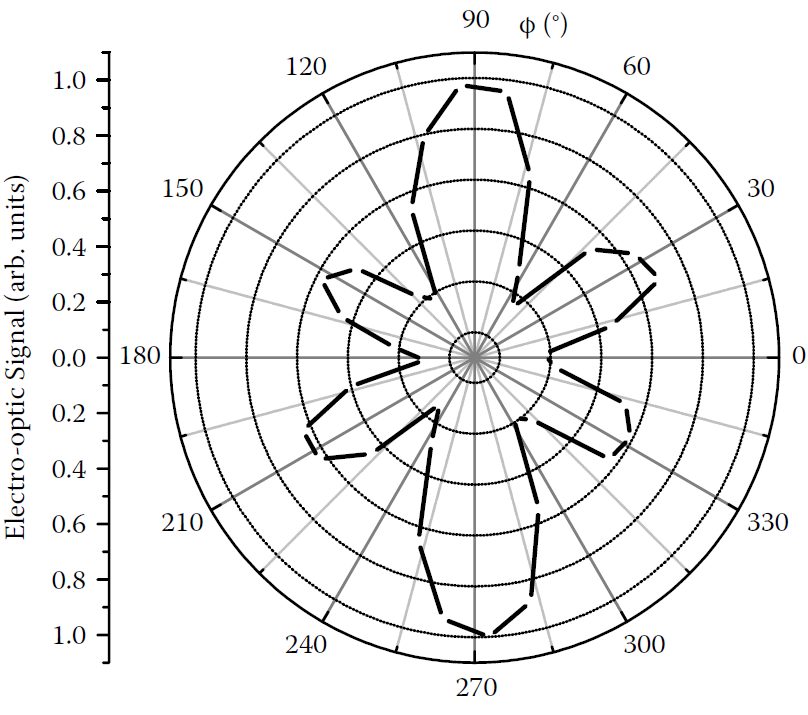
\includegraphics[width=0.6\textwidth]{refferenced_pic/degreedepenceZnTe.png}
    \caption{The plot shows the angle-dependent emission of $\si{\tera\hertz}$ radiation in ZnTe.
    The angle is between the $(001)$ direction of the crystal and the polarization of the pump beam. An angle of $\phi = \SI{90}{\degree}$ however relates to the pump beam polarization being parallel to the $(001)$ axis.
    The plot is taken from the source \cite{selig}.}
    \label{fig:polarization_dependence_angle}
\end{figure} \FloatBarrier
This effect is discussed in section \ref{sec:eos}.
The refractive index of ZnTe at $\SI{800}{\nano\meter}$ is $n_\text{ZnTe, 800\,nm} = 2.85$ \cite{refractive_index_znte}.
At a frequency of $\SI{1}{\tera\hertz}$ it is approximately  $n_\text{ZnTe, 1\,THz} = 3.17$ \cite{hebling2004tunable}.
This difference harms the generation of $\SI{1}{\tera\hertz}$ radiation in comparison to higher or lower frequencies.
The relationship between $\si{\tera\hertz}$ frequencies and coherence lengths can be seen in figure \ref{fig:coherence_legnth}.
\subsection{Gallium phosphide}
The other crystal used to generate $\si{\tera\hertz}$ radiation is gallium phosphide (GaP).
It is a common emitter of $\si{\tera\hertz}$ radiation with a broad spectrum.
This crystal also exhibits a phonon resonance, but at a much higher frequency of about $\SI{11}{\tera\hertz}$ \cite{phonon_GaP}.
As well as ZnTe, GaP needs to be stimulated by the laser along its $(110)$ axis.
The refractive index of GaP at $\SI{800}{\nano\meter}$ is $n_\text{GaP, 800\, nm} = 3.193$ \cite{refractive_index_gap}.
At $\SI{1}{\tera\hertz}$ the refractive index is $n_\text{GaP, 1\,THz} = 3.34$ \cite{hebling2004tunable}.
%%%%%%%%%%%%%%%%%%%%%%%%%%%%%%%%%%%%%%%%%%%%%%%%%%%%%%%%%%%%%%%%%%%%%%%%%%%%%%%%%%


%%%%%%%%%%%%%%%%%%%%%%%%%%%%%%%%%%%%%%%%%%%%%%%%%%%%%%%%%%%%%%%%%%%%%%%%%%%%%%%%%%
\section{Optical rectification}\label{sec:optic_ref}
To generate $\si{\tera\hertz}$ radiation advantage is taken of optical rectification or rather a kind of difference frequency mixing that is very similar to optical rectification.
Optical rectification is a second-order non-linear effect and thus can be just observed in non-linear materials.
This effect causes a DC polarization in the crystal \cite{wiki_book}.
If the DC polarization is modulated correctly it will cause $\si{\tera\hertz}$ radiation.
The DC polarization occurs when an electric field interacts with the crystal.
To discuss the effect in detail the effect of the electric field on the polarization needs to be looked at.
The polarization is defined as
\begin{equation}
P = \chi(E) E \epsilon_0\, ,
\end{equation}
where $\epsilon_0$ is the vacuum permittivity.
The polarization is directly proportional to the electric field $E$ and the susceptibility $\chi(E)$, which can than be expanded to 
\begin{equation}
    \chi(E) = \chi_1 + \chi_2 E +\chi_3 E^2 + ...   \, .
\end{equation}
As described earlier, optical rectification is a second-order effect and is described by the $P_\text{nl} = \epsilon_0\chi_2 E^2$ term.
Because the laser generates electromagnetic radiation at the whole bandwidth of frequencies $\omega + \symup{\Delta}\Omega$, in a gaussian profile, it is necessary to consider all of those electric fields mixing inside the crystal.
To simplify it is best to look at just two electric fields first.
One of those electric fields oscillates at frequency $\omega_\text{i}$ and the other at frequency $\omega_\text{j}$.
The two electric fields can then be writen as $E_\text{i} = E_0\cos(\omega_\text{i} t)$ and $E_\text{j} = E_0\cos(\omega_\text{j} t)$ with the same amplitude $E_0$.
The resulting second-order polarization term 
\begin{equation}
    P_\text{nl} = \chi_2 \epsilon_0 \frac{E_0^2}{2}\left[\cos((\omega_\text{i} - \omega_\text{j})t) + \cos((\omega_\text{i} + \omega_\text{j})t)\right]
\label{eq:two_freq_mixing}
\end{equation}
shows a cosine with a difference dependency $\omega_\text{i}-\omega_\text{j}$ and one with a sum dependency $\omega_\text{i}+\omega_\text{j}$.
The one with the difference dependency results in the generation of $\si{\tera\hertz}$ radiation. % the one with the sum depends is important for second harmonic generation
The sum term of equation \eqref{eq:two_freq_mixing}, results in second-harmonic generation \cite{boyd2020nonlinear} and is not important for $\si{\tera\hertz}$ generation and will be neglected in further calculations \cite{wiki_book}.
If the whole bandwidth $\omega + \symup{\Delta}\Omega$ is now taken into account, all the frequencies interact with the crystal.
This results in a polarization dependency on all the frequencies $\symup{\Delta}\Omega$ in the bandwidth as such
\begin{equation}
    P_{\symup{\Delta}\Omega} = \chi_2 \epsilon_0 \frac{E_0^2}{2}\cos(\symup{\Delta}\Omega t) \, .
    \label{eq:polarization_depens}
\end{equation}
With the right bandwidth, the resulting change in polarization generates $\si{\tera\hertz}$ radiation \cite{book_optical_rectification,wiki_book}.
\\\\
The process of $\si{\tera\hertz}$ generation can also be explained by the excitation of higher energy levels.
It is visualized in figure \ref{fig:freq_mix}.\FloatBarrier
\begin{figure}
    \centering
    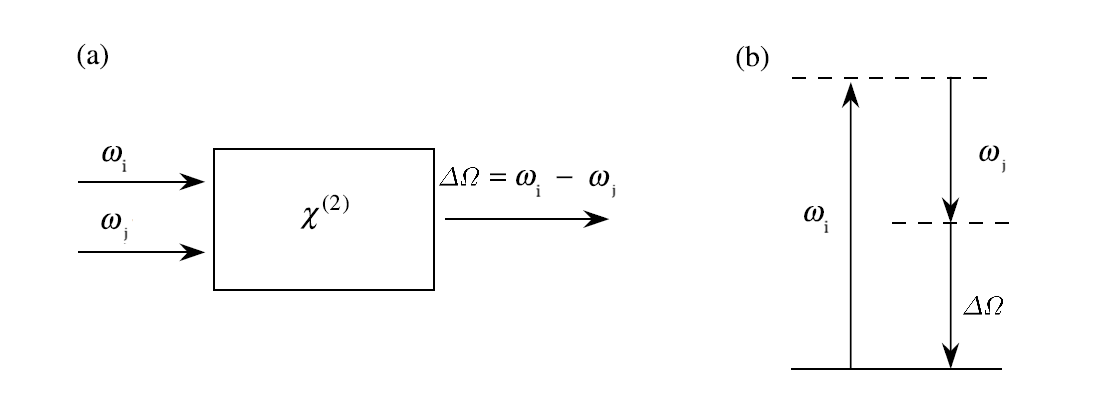
\includegraphics[width=\textwidth]{refferenced_pic/diffrence_frequency_mixing.PNG}
    \caption{Figure (a) shows the two fields with frequencies $\omega_\text{i} $ and $\omega_\text{j}$ going into the non-linear medium with susceptibility $\chi_2$.
    Through difference frequency mixing the medium emits radiation at frequency $\symup{\Delta}\Omega$.
    Figure (b) shows the interaction of frequency $\omega_\text{i} $ and $\omega_\text{j}$ inside the medium.
    Here $\omega_\text{i}$ excites a higher virtual energy level, from which $\omega_\text{j}$ gets substracted which leaves $\symup{\Delta}\Omega$.}
    \label{fig:freq_mix}
\end{figure}\FloatBarrier
A field with frequency $\omega_\text{i}$ goes into the crystal excites a higher energy level.
Now another field  with frequency $\omega_\text{j}$ goes into the crystal excites a two-photon emission that in turn lowers the energy level again but not to the ground state.
There can also occur a spontaneous two-photon emission without the presence of the frequency $\omega_\text{j}$ however, its probability is way lower.
From the lower energy level, the system then drops back to the ground state.
Because of the conservation of energy, the crystal puts out a photon of the difference
\begin{equation}
    \symup{\Delta}\Omega = \omega_\text{i} - \omega_\text{j} \, ,
\end{equation}
where $\omega_\text{i}$ corresponds to the higher and $\omega_\text{j}$ to the lower energy level.
With the right input frequencies, the difference result is in the $\si{\tera\hertz}$ regime \cite{boyd2020nonlinear}.
%%%%%%%%%%%%%%%%%%%%%%%%%%%%%%%%%%%%%%%%%%%%%%%%%%

%Hier noch Grafik rein und vielleicht nochmal was ändern
%Patrick hat das ganze ja eher durch das anregen von virtuellen Energielevel erklärt.
%Dazu wäre eine Grafik auch gut

%%%%%%%%%%%%%%%%%%%%%%%%%%%%%%%%%%%%%%%%%%%%%%%%%%

\section{Electro-optic sampling}\label{sec:eos}
To detect the $\si{\tera\hertz}$ electric field electro-optic sampling (EOS) is used.
Which makes use of the electro-optic effect also known as the Pockels effect.
Through this effect, a birefringence is induced in the detection crystal which in turn changes the polarization of the probe beam.
The phase shift 
\begin{equation}
    \text{sin}(\theta) = \frac{2\pi}{\lambda} n_0^3 l r E_\text{THz}
\end{equation}
is directly proportional to the electric field $E_\text{THz}$. 
It is also proportional to the crystal thickness $l$, the electro-optic coefficient $r$, and the refractive index $n_0$ and inversely proportional to the wavelength $\lambda$ \cite{wiki_book}. 
Through measurement of the change in polarization, it is then possible to determine the electric field strength of the $\si{\tera\hertz}$-pump beam.
For this, the difference in intensity of the horizontally and vertically polarized part of the beam $\symup{\Delta}I$ is measured.
It is explained in section \ref{sec:setup} how the beam is split into its two polarization-dependent parts and how the intensities are then measured.
With the normed difference 
\begin{equation}
    \frac{\symup{\Delta}I}{I} = \text{sin}(\theta) = \frac{2\pi}{\lambda} n_0^3 l r E_\text{THz}
    \label{eq:electricfield_A_B}
\end{equation}
of the intensities over the whole intensity $I$ it is then possible to determine the field strength $E_\text{THz}$ \cite{THZ_eltric_field}.
With the electric field calculated, the peak power of the $\si{\tera\hertz}$ electric field is then attainable.
For this the intensity
\begin{equation}
    I_\text{THz} = c \epsilon_0 E_\text{THz}^2
    \label{eq:intensity}
\end{equation}
of the $\si{\tera\hertz}$ electric field is calculated.
The power 
\begin{equation}
    P = \int\, I_\text{THz} \,\symup{d}A_\text{spot}
\end{equation}
can then be obtained by integrating the intensity $I_\text{THz}$ over the area of the $\si{\tera\hertz}$ spot $A_\text{spot}$ \cite{griffiths}.
Because it is not possible to measure the distrubution of the intensity in this setup, an equally distributed intensity has to be assumed.
With this the equation simplifies to 
\begin{equation}
    P = I_\text{THz}A_\text{spot}\,.
    \label{eq:power}
\end{equation}
With the power of the electric field, a conversion efficiency $C$ can be calculated by formula
\begin{equation}
    C = \frac{P_\text{THz}}{P_\text{pump}} \, ,
    \label{eq:conversion}
\end{equation}
in which $P_\text{THz}$ is the peak electric field power and $P_\text{pump}$ is the pump power.
%%%%%%%%%%%%%%%%%%%%%%%%%%%%%%%%%%%%%%%%%%%%%%%%%%%%%%%%%%%%%%%%%%%%%%%%


%%%%%%%%%%%%%%%%%%%%%%%%%%%%%%%%%%%%%%%%%%%%%%%%%%%%%%%%%%%%%%%%%%%%%%%%
\section{Coherence length}
\label{sec:coherence_length}
As mentioned in section \ref{sec:emitters} the refractive index of the crystal at the laser frequency and the $\si{\tera\hertz}$ frequencies have a great impact on the generation of $\si{\tera\hertz}$ radiation.
Because the refractive indices of the $\SI{800}{\nano\meter}$ laser pump beam and the generated $\si{\tera\hertz}$ radiation generally differ from one another, the pulses travel at different speeds inside the crystal.
If the mismatch is too big the efficiency of generation and detection of $\si{\tera\hertz}$ radiation through the crystals suffers.
The effective length at which the velocity mismatch can be tolerated is called the coherence length
\begin{equation}
    l(\omega_{\si{\tera\hertz}}) = \frac{\pi c}{\omega_{\si{\tera\hertz}} \left | n_\text{opt eff}(\omega_0) - n_{\si{\tera\hertz}}(\omega_{\si{\tera\hertz}})\right |}
\end{equation}
with 
\begin{equation}
    n_{\text{opt eff}} = n_\text{opt}(\omega) - \lambda_\text{opt}\frac{\partial n_\text{opt}}{\partial \lambda}\biggl{|}_{\lambda_\text{opt}} \, .  
\end{equation}
Here $\omega_{\si{\tera\hertz}} = 2\pi  \nu_{\si{\tera\hertz}}$ is the frequency of $\si{\tera\hertz}$ radiation, $\omega_0$ is the frequency of the laser, $n_{\si{\tera\hertz}}$ is the refractive index of $\si{\tera\hertz}$ radiation in the medium, $n_\text{opt}$ is the refractive index at the pump laser wavelength $\lambda_\text{opt}$ and $n_\text{opt eff}$ is the refractive index of the group velocity of the pump laser radiation in the crystal \cite{coherence_legnth}.
Because the refractive index of $\si{\tera\hertz}$ radiation and $\SI{800}{\nano\meter}$ laser light in ZnTe is similar for most $\si{\tera\hertz}$ frequencies up to $\SI{2.5}{\tera\hertz}$ \cite{coherence_legnth}, the coherence length for those frequencies is long enough for the application in the setup described in section \ref{sec:setup}.
The relation between coherence length and $\si{\tera\hertz}$ frequency in ZnTe is shown in figure \ref{fig:coherence_legnth}.
\\\\
GaP has a lower coherence length at $\SI{800}{\nano\meter}$ laser light and most $\si{\tera\hertz}$ frequencies.
Its coherence length in relation to the frequencies can be seen in figure \ref{fig:coherence_length_GaP}.
Its lower coherence length results in a bigger mismatch the longer the crystal.
For this reason, the chosen GaP crystal is thinner than the ZnTe crystal.
\begin{figure}
    \centering
    \begin{subfigure}{.5\textwidth}%
        \centering
        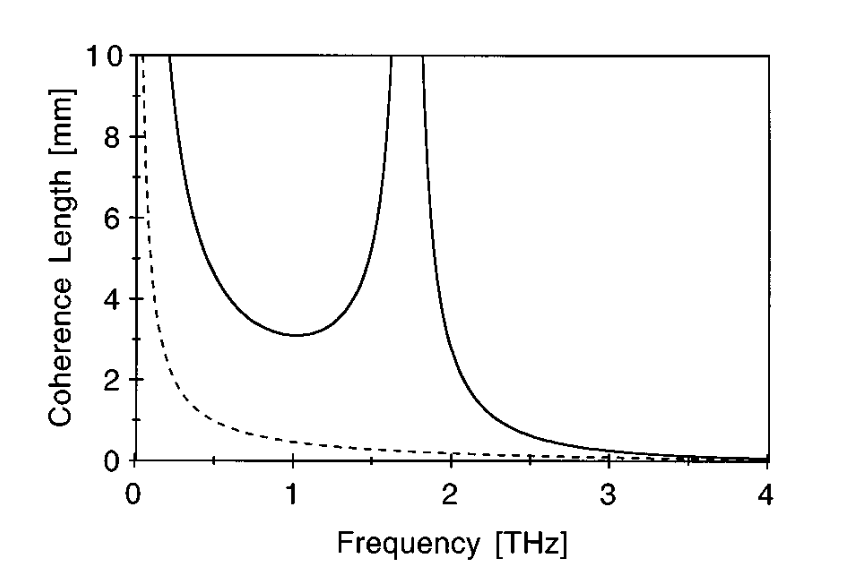
\includegraphics[width=\textwidth]{refferenced_pic/coherence_length_ZnTe.png}
        \caption{}
        %\caption{The coherence length of an $\SI{800}{\nano\meter}$ laser pulse and $\si{\tera\hertz}$ radiation in dependence on the $\si{\tera\hertz}$ frequency.
        %The solid line includes the effect of dispersion at optical frequencies. The dotted line neglects the dispersion at optical frequencies \cite{coherence_legnth}.}
        \label{fig:coherence_legnth}
    \end{subfigure}%
    \hfill
    \begin{subfigure}{.5\textwidth}%
        \centering
        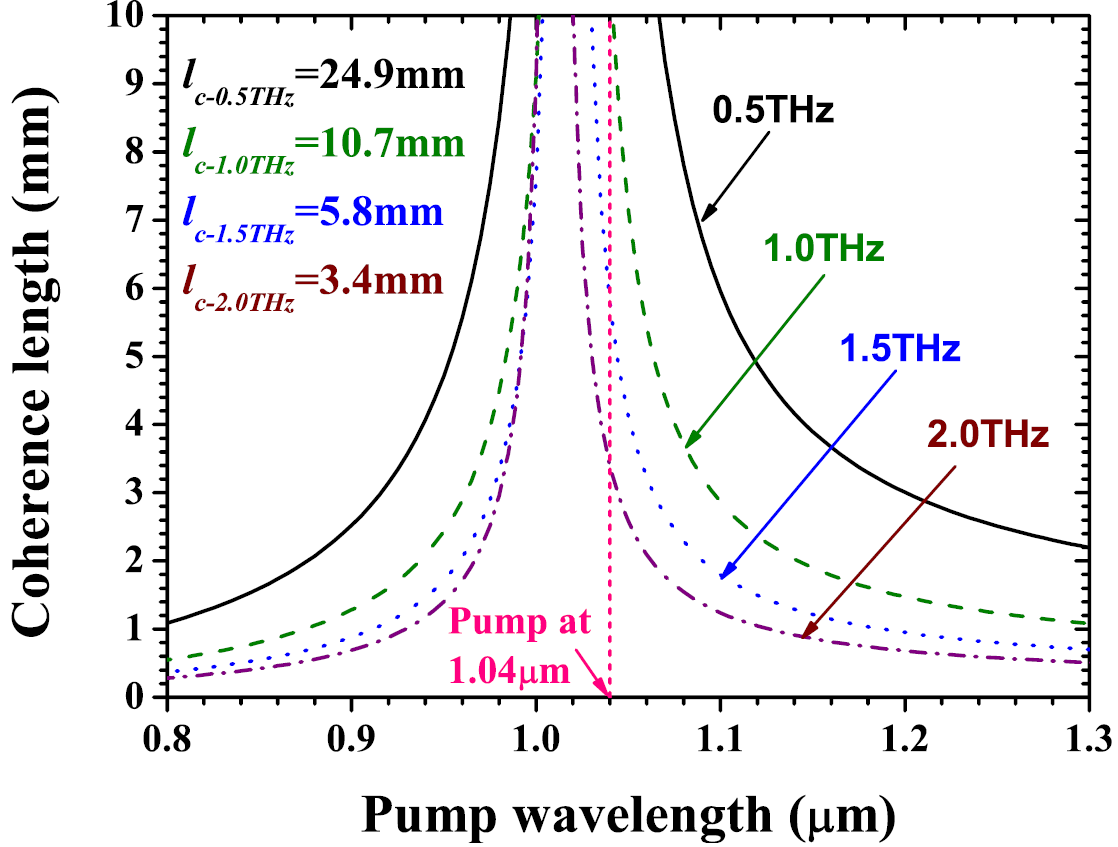
\includegraphics[width=\textwidth]{PLots/GAP_coherencelength.png}
        \caption{}
        %\caption{The coherence length of an $\SI{800}{\nano\meter}$ laser pulse and $\si{\tera\hertz}$ radiation in GaP, in dependence on the laser frequency.
        %Different $\si{\tera\hertz}$ frequencies are plotted to show their difference \cite{GaP_coherence_length}.
        %}
        \label{fig:coherence_length_GaP}
    \end{subfigure}%
    \caption{The left figure \ref{fig:coherence_legnth} shows the coherence length of an $\SI{800}{\nano\meter}$ laser pulse and $\si{\tera\hertz}$ radiation in dependence on the $\si{\tera\hertz}$ frequency.
    The solid line includes the effect of dispersion at optical frequencies. The dotted line neglects the dispersion at optical frequencies \cite{coherence_legnth}.
    The right figure \ref{fig:coherence_length_GaP} shows the coherence length of an $\SI{800}{\nano\meter}$ laser pulse and $\si{\tera\hertz}$ radiation in GaP, in dependence on the laser frequency.
    Different $\si{\tera\hertz}$ frequencies are plotted to show their difference \cite{GaP_coherence_length}.}
    \label{fig:coherence_length_both}
\end{figure}
% I need a paper to refernce the coherence length of GaP